%!TEX ROOT=formularioFisica.tex

\section{Relatività}
La relatività dà inisio alla Fisica moderna.\\
Grazie ad Einstein ma non solo, si è aperto un nuovo capitolo.

\subsection{Trasformazioni Galileiane}
Si distinugono due tipi di sistemi di riferimento:
\textbf{inerziali} che soddisfano il principio di inerzia di Newton e \textbf{non inerziali} che
invece non lo soddisfano.\\
Un sistema che si muove di Moto Rettilineo Uniforme rispetto ad un altro sistema inerziale. È 
anch'esso inerziale. Andiamo a disegnare questi due sistemi inerziali.
\begin{center}
  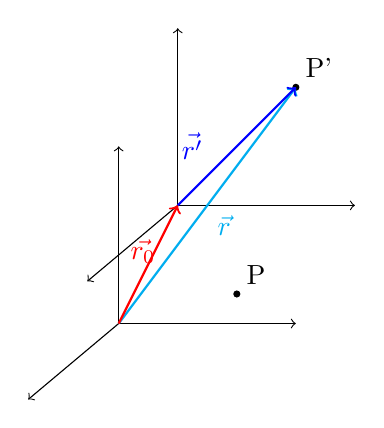
\begin{tikzpicture}[scale=0.75]
    \coordinate (O) at (0,0);
    \coordinate (O') at (1,2);
    \coordinate (P) at (2,0.5);
    \coordinate (P') at (3,4);

    \draw[->] (O) -- ++(0,3);
    \draw[->] (O) -- ++(3,0);
    \draw[->] (O) -- ++(220:2);

    \draw[->] (O') -- ++(0,3);
    \draw[->] (O') -- ++(3,0);
    \draw[->] (O') -- ++(220:2);
    
    \filldraw (P) circle (0.05);
    \filldraw (P') circle (0.05);

    \draw[->, thick,cyan] (O) -- (P')
      node[pos=0.5,below right]{$\vec{r}$};
    \draw[->, thick,blue] (O') -- (P')
      node[pos=0.3,above left]{$\vec{r'}$};
    \draw[->, thick,red] (O) -- (O')
      node[pos=0.8, below left]{$\vec{r_0}$};
    %\draw[->, thick] (P) -- (P')
    %  node[pos=0.5,right]{$\vec{v}$};

    \node[above right] at (P){P};
    \node[above right] at (P'){P'};
  \end{tikzpicture}
\end{center}
In $t=0$, si ha che $S$ e $S'$ coincidono.\\
All'istante $t_1\,(t_1\neq0)$ si ha che
\begin{equation*}
  \vec{r_1} = \vec{r_1'} + \vec{v}t_1
\end{equation*}
All'istante $t_2\,(t_2\neq0)$ si ha che
\begin{equation*}
  \vec{r_2} = \vec{r_2'} + \vec{v}t_2
\end{equation*}
Trovando la differenza
\begin{equation*}
  \Delta \vec{r} = \Delta\vec{r'}+\vec{v}\Delta t
\end{equation*}
Dividendo per $\Delta t$
\begin{equation*}
  \frac{\Delta\vec{r}}{\Delta t}=\frac{\Delta\vec{r'}}{\Delta t}+\vec{v}
\end{equation*}
si ottiene
\begin{equation*}
  \vec{u} = \vec{u'}+\vec{v}
\end{equation*}
E questa è chiamata la \textbf{legge di composizione delle velocità}. Si ricordi che tutto ciò che
ha un apice (come $u'$) è relativo al sistema di riferimento $S'$.\\ [\baselineskip]
Imposto che $S'$ si muova di moto rettilineo uniforme sull'asse delle $x$ di $S$, le trasformazioni
galileiane sono così descritte
\begin{equation*}
  \begin{cases}
    x' = x-vt\\
    y'=y\\
    z'=z\\
    t'=t
  \end{cases}
\end{equation*}
L'ultima equazione è la più importante in questo caso. Essa infatti ci dice che \textbf{il tempo è
assoluto e non dipende dal sistema di riferimento}. 

\subsection{Esperimento di Michelson-Morley}
Nell'arco di venti e più anni, i due scienziati Michelson e Morley dimostrarono che la velocità della
luce non variava e che quindi il vento dell'etere, precedentemente teorizzato per conciliare 
meccanica classica e studio della luce, non esisteva.
\subsubsection{Il vento dell'etere}
L'esperimento del vento dell'etere può essere riassunto così
\begin{center}
  \begin{tikzpicture}[square/.style={regular polygon,regular polygon sides=4}]
    \coordinate (A) at (0,0);
    \coordinate (B) at (3,0);
    \coordinate (C) at (0,3);

    \node at (A) [square,draw](A){A};
    \node at (B) [square,draw](B){B};
    \node at (C) [square,draw](C){C};

    \draw[|<->|] (A) -- (B)
      node[pos=0.5,below]{$L$};
    \draw[|<->|] (A) -- (C)
      node[pos=0.5,left]{$L$};

    \foreach\y in {2,1.5,1}{%
      \draw[->] (3,\y) -- ++(-2,0);
    }
  \end{tikzpicture}
\end{center}
Definendo $v_M$ la velocità del moto e $v_V$ la velocità del vento, si può immaginare un corpo che
segue la rotta A-B e un altro che segue quella A-C. La teoria dice che i tempi impiegati dai due 
moti devono essere diversi se il vento dell'etere esistesse. Infatti si ha che
\begin{equation*}
  t_\perp<t_\|
\end{equation*}
e questo verifica la tesi.\\ [\baselineskip]
Essendo l'etere solidale al sole, le due velocità perpendicolari e parallele dovevano essere
diverse. Ma, attraverso un interferometro che hanno continuato a migliorare, hanno dimostrato che
$c$ è sempre costante, non è mai cambiata. Infatti la Terra ruotando doveva intercettare l'etere
in maniere diverse. Questo avrebbe dovuto causare nell'interferometro diverse configurazioni di
interferenza ma questo non si è mai visto.

\subsection{Principi fondamentali della relatività ristretta}
La prima forumulazione della relatività si fonda su due principi cardine:
\begin{enumerate}
  \item \textbf{Tutte le formule devono avere la stessa forma per ogni tipo di sistema inerziale}
  \item \textbf{La luce nel vuoto ha la stessa velocità per ogni sistema} 
\end{enumerate}

\subsection{Simultaneità}
Einstein propone un esperimento mentale per illustrare che due eventi non sono simultanei se si tiene
conto dei principi della relatività. Infatti si immaginino due osservatori, $O$ su di una banchina
e $O'$ su di un treno in moto rettilineo uniforme rispetto a $O$ di velocità $\vec{v}$. Se 
$\vec{v}=\vec{0}$ ovviamente due qualsiasi eventi $E_1,E_2$ sarebbero simultanei per i due 
osservatori in quanto essi sarebbero nello stesso identico luogo.\\
Nel caso in cui però $\vec{v}\neq\vec{0}$, i due eventi non lo sono più. Infatti se esattamente 
quando $O\equiv O'$ si fanno partire due raggi luminosi a distanza uguale a destra e sinistra di $O$,
$O$ li vedrà arrivare nello stesso momento in quanto ha la stessa distanza da entrambi. $O'$ invece,
muovendosi, nel tempo che la luce impiega per raggiungerlo, avrà fatto un certo percorso e quindi 
vedrà i raggi in momenti diversi. $E_1$ ed $E_2$ non sono più simultanei per lui. Lo sarebbero se
$c=\infty$ ma è stato dimostrato che non è così.\\
Questo porta a due conseguenze
\begin{enumerate}
  \item \textbf{La dilatazione del tempo}
  \item \textbf{La contrazione della misura nella direzione del moto} 
\end{enumerate}

\subsection{Dilatazione del tempo}
Un orologio luminoso è composto da una sorgente luminosa posta ad un'estremità di una scatola di 
lunghezza $l$ e da uno specchio nell'altra. L'unità di tempo diventa quindi il tempo necessario alla
luce ad andare e tornare.\\
Si prendano due osservatori, $O$ su di una banchina e $O'$ su di un treno che si muove di velocità
$\vec{v}$ rispetto a $O$. Entrambi hanno un orologio luminoso. Si definisca $\Delta t'$ il tempo
misurato dall'orologio di $O$. Esso sarà pari a
\begin{equation*}
  \Delta t' = \frac{2l}{c}
\end{equation*}
Il tempo $\Delta t$ invece sarà diverso in quanto nel periodo in cui la luce raggiunge lo specchio,
il treno con l'ossevatore $O'$ si sarà spostato. Quindi si ha una situazione del genere
\begin{center}
  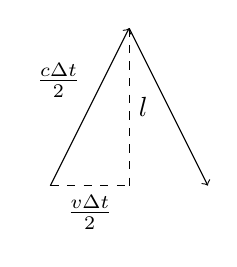
\begin{tikzpicture}
    \draw[->] (0,0) -- (1,2)
      node[pos=0.5,above left]{$\frac{c\Delta t}{2}$};
    \draw[->] (1,2) -- (2,0);
    \draw[dashed] (1,2) -- (1,0)
      node[pos=0.5,right]{$l$};
    \draw[dashed] (0,0) -- (1,0)
      node[pos=0.5,below]{$\frac{v\Delta t}{2}$};
  \end{tikzpicture}
\end{center}

\begin{equation*}
  {\left( \frac{c\Delta t}{2} \right)}^2=l^2+{\left( \frac{v\Delta t}{2} \right)}^2
\end{equation*}
Risolvendo e mettendo a sistema si ottiene
\begin{equation*}
  \Delta t = \frac{\Delta t'}{\sqrt{1-\frac{v^2}{c^2}}}
\end{equation*}
Quindi abbiamo che $\Delta t\neq\Delta t'$. Anzi, per $v\ll c$ si ha che $\Delta t \to \Delta t'$.
$\Delta t'$ viene definito \textbf{tempo proprio}. Il termine
\begin{equation*}
  \gamma = \frac{1}{\sqrt{1-\frac{v^2}{c^2}}}
\end{equation*}
tornerà spesso fuori anche nelle trasformazioni di Lorentz, non è un caso si ritrovi anche lì.

\subsection{La velocità limite della luce}
Se si prende il fattore $\gamma$ e lo si studia, si capirà subito che non può esserci una velocità
maggiore $c$. Andando a fare un semplice studio di funzione si vede che, andando a calcolare la 
derivata prima si trova
\begin{equation*}
  \der{\gamma(v)}{v} = \frac{v \left( 1-\frac{v^2}{c^2} \right)}{c^2\sqrt{1-\frac{v^2}{c^2}}}
\end{equation*}
Andando a studiare il segno vediamo che in $v=0$ ha un minimo. $\gamma(0)=1$.
Infine andando a fare il limite
\begin{equation*}
  \lim\limits_{v\to c^-} \gamma = +\infty 
\end{equation*}
si vede che $v=c$ è asintoto verticale e che quindi non è possibile superare la velocità della 
luce.\\
Poiché
\begin{equation*}
  \frac{\Delta t}{\Delta t'}=\gamma > 1
\end{equation*}
si verifica l'esistenda di una \textbf{dilatazione temporale}.

\subsection{Trasformazioni di Lorentz}
Le trasformazioni di Lorentz hanno la caratteristica di rendere invarianti le equazioni di Maxwell.
Presi due sistemi inerziali $S$ e $S'$ che si muovono sull'asse delle $x$ di moto rettilineo 
uniforme, le trasformazioni di Lorentz si scrivono come
\begin{equation*}
  \begin{cases}
    x'= \gamma(x-vt)\\
    y'=y\\
    z'=z\\
    t'=\gamma(t-\frac{v}{c^2}x)
  \end{cases}
\end{equation*}
La grande ed enorme novità sta proprio nell'ultima equazione, quella relativa al tempo. Sono due 
tempi diversi che dipendono dalla posizione e dalla velocità.\\
Presi due istanti $t_1',t_2'$ si ha che
\begin{equation*}
  \Delta t = t'_2\gamma -\cancel{\frac{vx}{c^2}\gamma}-t'_1\gamma+\cancel{\frac{vx}{c^2}\gamma}=
  \gamma\Delta t'
\end{equation*}
Che è esattamente lo stesso risultato ottenuto da Einstein nei suoi esperimenti mentali.

\subsection{Contrazione delle lunghezze}
Presi due sistemi di riferimento $O,O'$ che si muovono di moto rettilineo uniforme tra di loro e un
corpo di lunghezza $L$ fermo per $O'$, i due sistemi misureranno $L$ per $S$ e $L'$ per $S'$. Si ha
\begin{equation*}
  O'\,\text{misurerà}\,L'= x_B'-x_A'\quad O\,\text{misurerà}\,L=x_B-x_A
\end{equation*}
Si ha inoltre che $x'=\gamma(x-vt)$. Calcolando allora
\begin{equation*}
  L' = x_B'-x_A'=\gamma(x_B-vt)-\gamma(x_A-vt)=\gamma(x_B-x_A)=\gamma L
\end{equation*}
Si ha quindi che
\begin{equation*}
  L = \frac{L'}{\gamma}
\end{equation*}
e che quindi le due lunghezze non sono misurate uguali dai due sistemi di riferimento.

\subsection{Piano di Minkowsky}
Minkowsky ha preso le trasformazioni di Lorentz e le ha guardate da un punto di vista puramente
matematico. Il suo piano è un piano di questo tipo
\begin{center}
  \begin{tikzpicture}
    \draw[->,thick] (-0.5,0) -- (3,0)
      node[pos=0.9,below]{$x$};
    \draw[->,thick] (0,-0.5) -- (0,3)
      node[pos=0.9,left]{$ct$};
  \end{tikzpicture}
\end{center}
Come mai $ct$ nell'asse delle $y$? Se un punto $P$ è definito da 4 variabili $P(x,y,z,t)$, non si
può avere tre unità di misura di lunghezza e una di tempo. Per uniformarle, si è moltiplicato il
tempo per una velocità (sempre costante), ottenendo una lunghezza.\\
Lo spazio quadridimensionale $\mathbb{R}^4$ è stato semplificato in $\mathbb{R}^2$ in quanto le
coordinate $y$ e $z$ sono costanti. Notiamo inoltre che il piano, rispetto alla fisica classica, 
ha invertiti tempo e posizione.\\ [\baselineskip]
Andando a scrivere le equazioni di Lorentz con $\beta = \frac{v}{c}$
\begin{equation*}
  \begin{cases}
    x' =\gamma(x-\beta ct)\\
    t'=\gamma\left(t-\beta\frac{x}{c}\right)
  \end{cases}
\end{equation*}
Per trovare l'asse verticale, poniamo $ct'=0$, $t'=0$ e che quindi $ct = \beta x$. Questo è il 
nuovo asse del piano di Minkowsky. Ponendo $x'=0$ si ha che $ct=\frac{x}{\beta}$ e che quindi 
abbiamo che la perpendicolare al primo-terzo quadrante è la retta che divide il piano. Praticamente
il piano ora diventa così
\begin{center}
  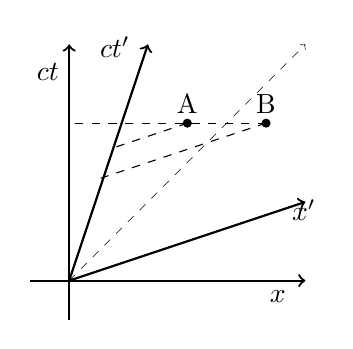
\begin{tikzpicture}
    \draw[->,thick] (-0.5,0) -- (3,0)
      node[pos=0.9,below]{$x$};
    \draw[->,thick] (0,-0.5) -- (0,3)
      node[pos=0.9,left]{$ct$};
    \draw[->,thick] (0,0) -- (1,3)
      node[pos=0.9,above left]{$ct'$};
    \draw[->,thick] (0,0) -- (3,1)
      node[pos=0.9,right]{$x'$};
    \draw[->,dashed,very thin] (0,0) -- (3,3);
    \filldraw (2.5,2) circle (0.05)
      node[above]{B};
    \filldraw (1.5,2) circle (0.05)
      node[above]{A};
    \draw[dashed] (2.5,2) -- (0,2);
    \draw[dashed] (2.5,2) -- (0.4,1.3);
    \draw[dashed] (1.5,2) -- (0.6,1.7);
  \end{tikzpicture}
\end{center}
Da questo vediamo una cosa che è fondamentale. $t_A=t_B$ ma $t'_A\neq t'_B$.

\subsection{Invariante spazio-temporale}
Minkowsky aveva trovato un'invariante nelle equazioni di Lorentz. Essa era $(\Delta\sigma)^2$. 
Infatti è definita come
\begin{equation*}
  {(\Delta\sigma)}^2={(c\Delta t)}^2-{(\Delta S)}^2
\end{equation*}
Dove $\Delta S$ è la differenza della variazione di tutte le coordinate.

\subsection{Causalità}
Come si può definire la causalità di due eventi se due osservatori li vedono in rapporti diversi?
\begin{center}
  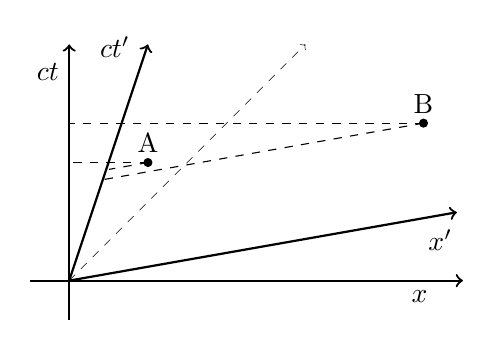
\begin{tikzpicture}
    \coordinate (A) at (1,1.5);
    \coordinate (B) at (4.5,2);
    \draw[->,thick] (-0.5,0) -- (5,0)
      node[pos=0.9,below]{$x$};
    \draw[->,thick] (0,-0.5) -- (0,3)
      node[pos=0.9,left]{$ct$};
    \draw[->,thick] (0,0) -- (1,3)
      node[pos=0.9,above left]{$ct'$};
    \draw[->,thick] (0,0) -- +(10:5)
      node[pos=0.9,below right]{$x'$};
    \draw[->,dashed,very thin] (0,0) -- (3,3);
    \filldraw (B) circle (0.05)
      node[above]{B};
    \filldraw (A) circle (0.05)
      node[above]{A};
    \draw[dashed] (B) -- (0,2);
    \draw[dashed] (A) -- (0,1.5);
    \draw[dashed] (B) -- +(10:-4.2);
    \draw[dashed] (A) -- +(10:-0.5);
  \end{tikzpicture}
\end{center}
Come possiamo vedere dall'esempio, secondo l'osservatore $S$, l'evento A viene prima di B, secondo
$S'$ invece è il contrario. Si ha che se 
\begin{equation*}
  \abs{x_B-x_A}\leq c\abs{t_B-t_A}
\end{equation*}
allora i due eventi si dicono \textbf{causalmente connessi}. In questo caso infatti si ha che
\begin{equation*}
  \left( \Delta\sigma \right)^2=\left( \Delta t \right)^2-\left( \Delta x \right)^2\geq0
\end{equation*}
In caso contrario (ovvero quando $(\Delta\sigma)^2<0$) i due eventi non sono causalmente legati.\\
Da questa caratteristica si possono dedurre alcune cose, tra le quali, cosa sia il presente, il
passato e il futuro.
\begin{center}
  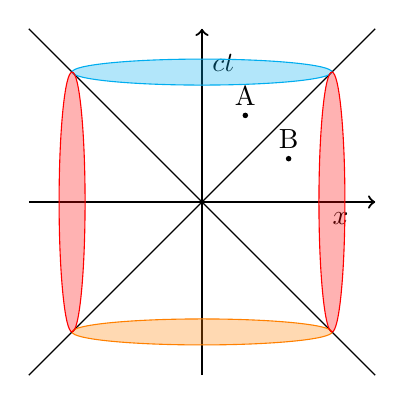
\begin{tikzpicture}[scale=0.55]
    \draw[thick,->] (-4,0) -- (4,0)
      node[pos=0.9,below]{$x$};
    \draw[thick,->] (0,-4) -- (0,4)
      node[pos=0.9,right]{$ct$};
    \draw (-4,-4) -- (4,4);
    \draw (-4,4) -- (4,-4);
    \filldraw[cyan,fill opacity=0.3] (0,3) ellipse (3 and 0.3);
    \filldraw[orange,fill opacity=0.3] (0,-3) ellipse (3 and 0.3);
    \filldraw[red,fill opacity=0.3] (3,0) ellipse (0.3 and 3);
    \filldraw[red,fill opacity=0.3] (-3,0) ellipse (0.3 and 3);
    \filldraw (1,2) circle (0.05)node[above] {A};
    \filldraw (2,1) circle (0.05)node[above] {B};
  \end{tikzpicture}
\end{center}
In questo grafico, A e B non sono causalmente connessi.\\
I coni le cui basi sono rosse sono denominati \textbf{coni del presente}. In questi coni, gli 
eventi non possono essere causalmente connessi a eventi futuri. Questo perché un corpo
dovrebbe muoversi ad una velocità maggiore di $c$ per poter rientrare nel cono del futuro.\\
Il cono con la base azurra è definito \textbf{cono del futuro}, quello con la base arancione
\textbf{cono del passato}. In questi coni, gli eventi possono essere causalmente connessi fra di 
loro per tutti gli osservatori, cosa che non accadeva negli altri.

\subsection{Dinamica relativistica}
La dinamica relativistica parte dalla nuova definizione di quantità di moto. Essa infatti da
$\vec{q}=m\vec{v}$ diventa
\begin{equation*}
  \vec{q} = m\gamma\vec{v}
\end{equation*}
In questo modo si mantiene il principio di conservazione della quantità di moto anche in ambito
relativistico.
\subsubsection{Lavoro}
Si prenda una particella di massa $m$ con $v_0=0$ su cui è applicata una forza $\vec{F}$ per farla
accelerare a velocità $v$. Se si definisce $1$ l'istante iniziale e $2$ quello finale,
il lavoro è pari a
\begin{equation*}
  L = \int\limits_{1}^{2} \vec{F}\dif\vec{r}=
  mc^2\gamma-mc^2
\end{equation*}
Notiamo quindi che l'energia cinetica di una particella ha due componenti. Viene definita
$E_0=mc^2$ l'energia a riposo, un'energia scoperta mai osservata prima d'ora che un corpo ha in 
virtù della sua massa. Si ha quindi che
\begin{equation*}
  E_0=mc^2\quad E_c=(\gamma-1)mc^2\quad E_{\text{tot}}=E_c+E_0=m\gamma c^2
\end{equation*}
\subsubsection{Rapporto quantità di moto-energia}
Si sa che $q=\gamma mv$ e $E=\gamma mc^2$. Si deduce che
\begin{equation*}
  E^2-c^2q^2=m^2c^4
\end{equation*}
Questo torna particolarmente utile nel caso in cui la particella in questione sia un fotone con
$m=0$. Si ha in tal caso
\begin{equation*}
  q=\frac{E}{c}
\end{equation*}
